\documentclass[12pt,twoside]{article}
\usepackage[basque]{babel}
\usepackage{graphicx}% Include figure files
\usepackage{multicol}

\input ../komandoak
\input ../logoak/watermark

\begin{document}

\izenburua{Ariketak. 8. gaia. Oszilazioak  }

\begin{enumerate}

\item 
Higidura harmonikoz plano horizontal batean eta segundoko bi
oszilazioz bibratzen ari den plataforma baten gainean kutxa bat
dago. Kutxaren eta plataformaren arteko marruskadura-koefiziente
estatikoak 0.5 balio du. Zein da oszilazioek izan dezaketen
anplituderik handiena, kutxak labain egin gabe jarraitzeko?
Plataformaren bibrazioa bertikala balitz, eta beraren anplitudea
$25\,{\rm mm}$-koa, zein izango litzateke maiztasunik handiena, kutxa
plataformatik alde ez egiteko?


\item 
\raisebox{-0.3cm}{
\begin{minipage}{0.7\linewidth}
 Partikula bat aurrerantz eta atzerantz labaintzen ari da, irudiko bi
planoen artean, marruskadurarik gabe.
\end {minipage}
\begin{minipage}{0.3\linewidth}
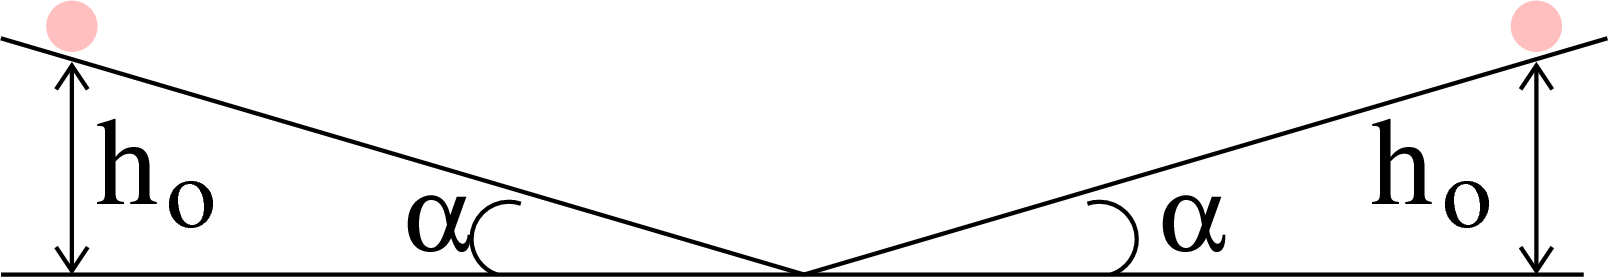
\includegraphics[width=\linewidth]{irudiak/08a-orria-biplano.png}
\end {minipage}
}
\begin{enumerate}
\item Lor bedi higiduraren periodoa, hasierako altuera $h_0$ baldin bada.
\item Higidura hori oszilakorra al da? Harmoniko sinplea al da?
\end{enumerate}

\item 
 Demagun bertikalki kokaturik dagoen malguki bati loturiko $m$ masako
partikularen oreka-posizio egonkorreko luzapena $l$ dela. Froga bedi sistema
perturbatuz gero $l$ luzerako pendulu sinplearena bezalako higidura oszilakorra
gauzatzen dela.


\item 
\raisebox{-0.7cm}{
\begin{minipage}{0.7\linewidth}
 Lor bedi $k_1$ eta $k_2$ errekuperazio-konstanteko malgukiez
osaturiko sistemaren errekuperazio-konstante baliokidea, malgukiak paraleloz
nahiz seriez elkarturik daudenean, irudian adierazten den bezala.
\end {minipage}
\hspace*{0.5cm}
\begin{minipage}{0.2\linewidth}
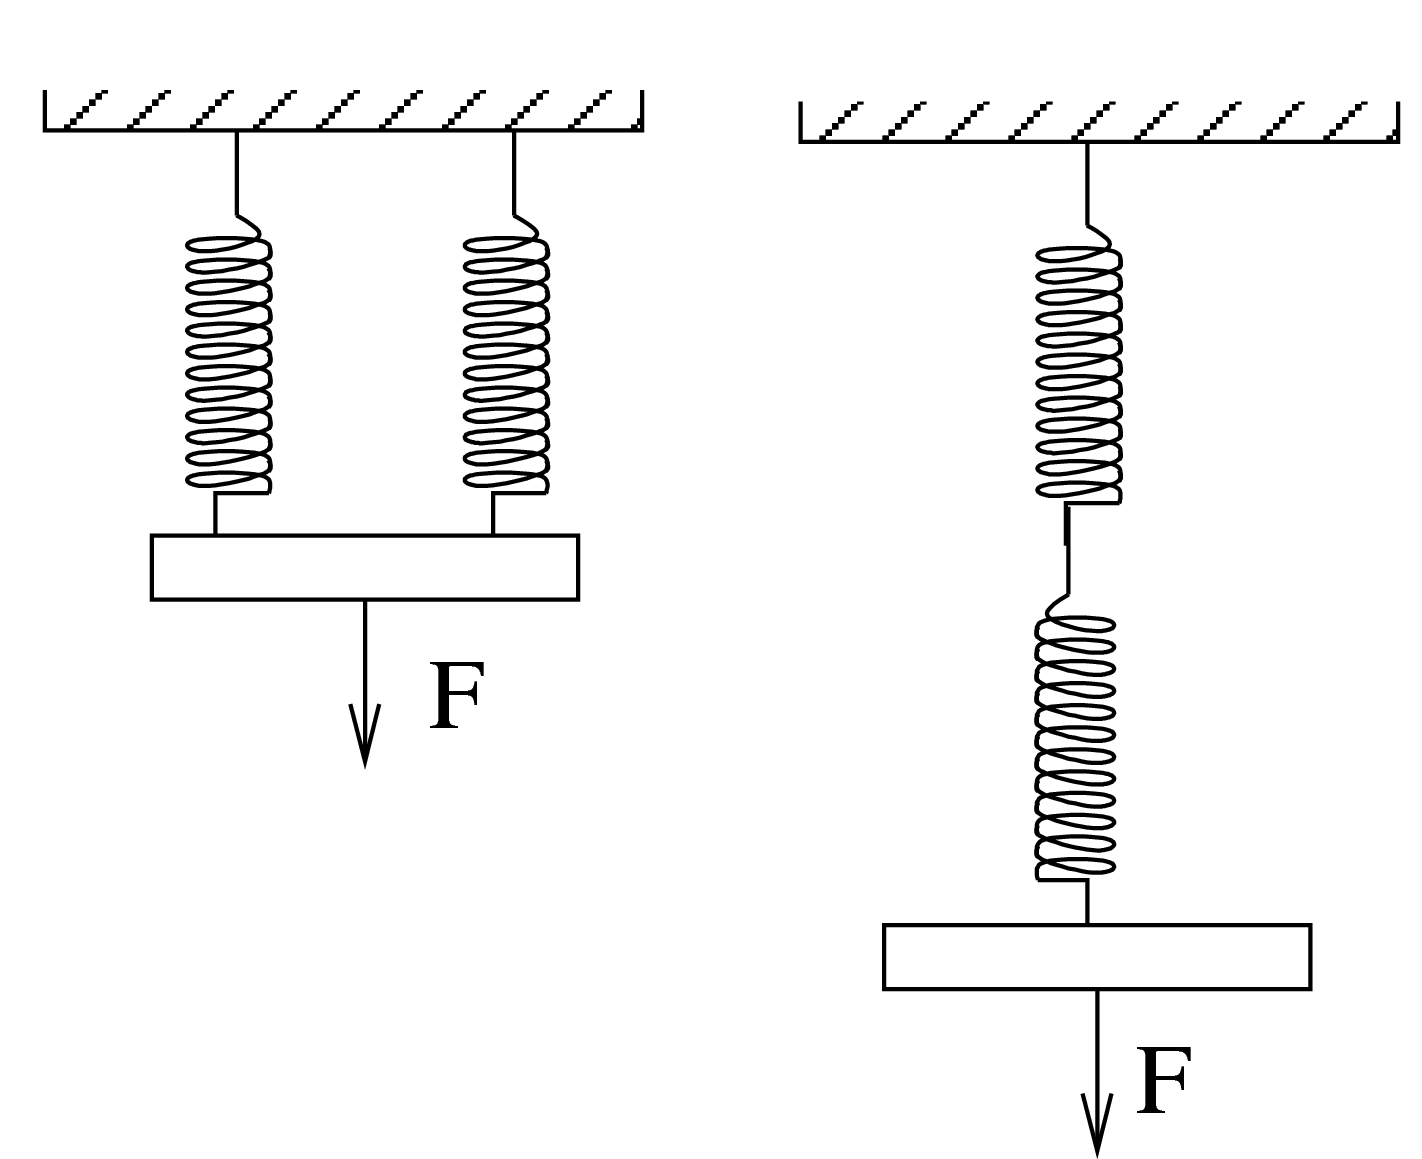
\includegraphics[width=\linewidth]{irudiak/08a-orria-malgukiser.png}
\end {minipage}
}


\item
2 kg-ko partikula bertikala den eta lurrari lotuta dagoen malguki baten
 muturrean dago.
 Malgukiaren luzera propioa 8~cm da, baina partikula bere gainean 
jartzean, malgukiaren luzera 5~cm da. Oreka-posizioan dagoenean, mailu batez 
beheranzko kolpe bat ematean, partikularen hasierako abiadura 0.3~m/s da. 
\begin{enumerate}
\item Zein izango da masak lortuko duen altuera maximoa?
\item Zenbat denbora  behar du masak lehenengo aldiz altuera maximoa 
lortzeko?
\item  Konprimatu barik egongo al da malgukia aldiuneren batean?
\item Hasierako aldiunean, zein da masak izan behar duen abiadura minimoa,
 aldiune batean bederen, malgukia konprimatu barik izan dadin? 
\end{enumerate}

\item
Oszilatzen duenean, malguki horizontal bati lotuta dagoen masaren periodoa 
T=4~s
da. Malgukia eta masa bertikalean eskegi ondoren, eta oszilatu barik, zein 
izango
 da malgukiak jasango duen luzapena?

\item
40 g-ko masa   puntualak T=0.32~s periodoa duen
 higidura harmoniko sinplea egiten du. Zein da anplitudearen balioa, 
higidura  sortzen duen indarraren balio maximoak 10 N balio badu.

\item
Paralelepipedo itxura duen zurezko blokearen dimentsioak eta 
dentsitate erlatiboa (blokearen dentsitatea/urarena) $a$, $b$, $c$
 eta $\rho_r$ dira hurrenez hurren.
 Blokea ur gainean dago, $a$ luzerako aldea bertikala izanik. 
Oreka-posizioan dagoenean beheranzko kolpe txiki bat eman ondoren, 
egiaztatu sortutako higidura harmonikoa dela. 
Kalkulatu oszilazioen maiztasun angeluarra. Marruskadura  arbuiatu.
Pista: Idatzi Newtonen bigarren legea blokearen higidura deskribatzeko.

\item
2~kg-ko gorputz batek 10~cm luzatzen du malguki bat orekan bertikalki
eskegita dagoenean. Gorputza malguki berberari lotzen zaio, baina
orain sistema marruskadura gabeko mahai baten gainean jarri da,
horizontalean, malgukiaren beste muturra puntu finko bati
lotuta. Oreka posiziotik 5~cm baztertzen da eta t=0 denean askatu
egiten da.
\begin {enumerate}
\item Aurkitu $A$ anplitudea, maiztasun angeluarra, maiztasuna eta
periodoa.
\item Zein da gorputzaren abiadura maximoa? Noiz lortzen da abiadura hori?
\item Ezaugarri berdinak dituen beste malguki bati 2~kg-ko beste masa
  bat lotzen zaio norabide horizontalean baina oraingoan 10~cm
  luzatzen da. Zein gorputz helduko da arinago oreka posiziora
  lehendabiziko aldiz? Zergatik?
\item Berriro gorputza oreka posiziotik baztertzean, hasierako posizioa
$3~$cm bada eta hasierako abiadura $-25~$cm/s,
 zein da oszilazioaren anplitudea eta 
hasierako fasea?
\end{enumerate}

\item
$M$ masa batek, hiru indar erakarle pairatzen ditu: 
Lehenengoa $OY$ ardatzaren perpendikularra da eta  $k_1\,x$ balio du.
Bigarrena $OX$ ardatzaren perpendikularra da eta  $k_1\,y$ balio du.
Hirugarrena $O$-rantza zuzenduta dago eta $k_2\,r$ balio du, 
$r$ koordenatu-jatorrira dagoen distantzia izanik.
$k_1$ eta $k_2$ delakoen balioak konstanteak dira. Masaren hasierako posizioa
 (0,$a$) bada eta hasierako abiadura, $v_0$, $OX$ ardatzaren paraleloa, aurkitu:

\begin{minipage}{.49\linewidth}

\begin{center}
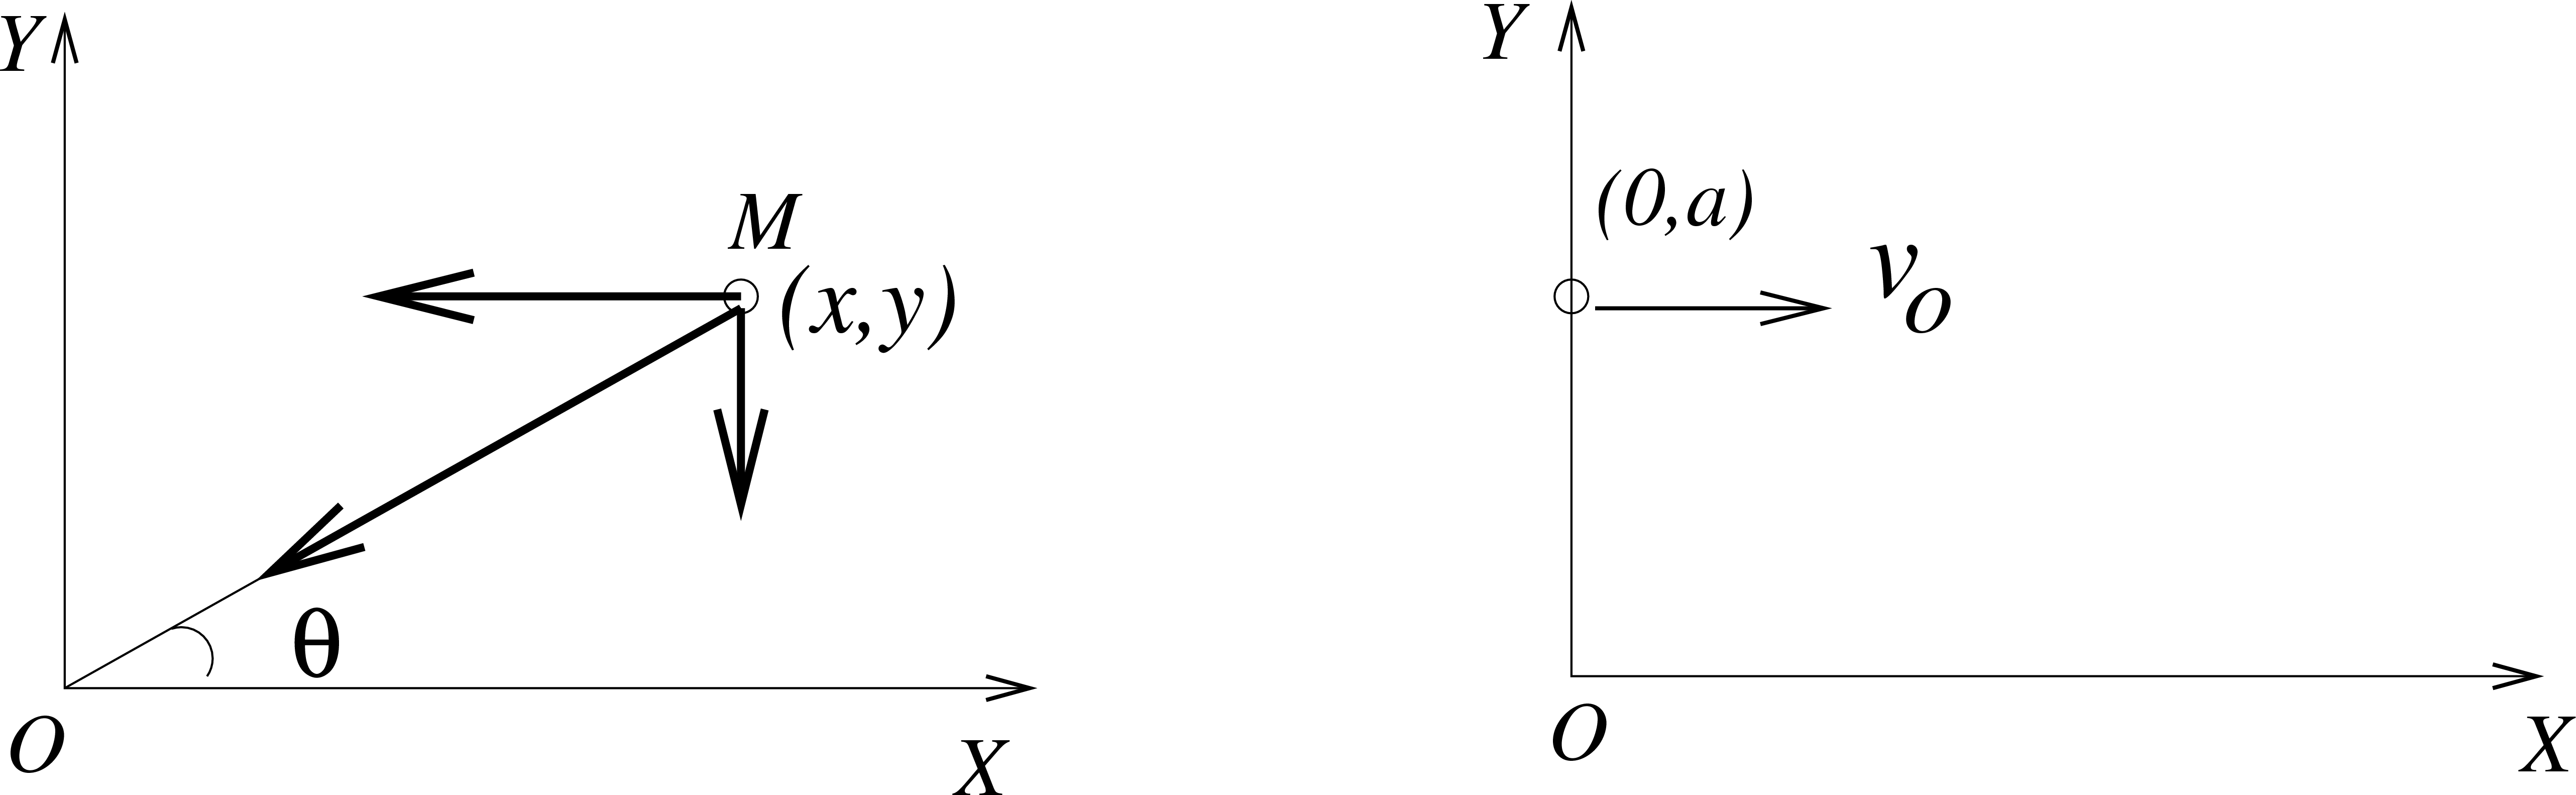
\includegraphics [width=\linewidth]{irudiak/3indar.png}
\end {center}
\end {minipage}\hfill
\begin{minipage}{.49\linewidth}
\begin{enumerate}
\item Higidura mota eta higiduraren periodoa
\item Higiduraren ekuazio parametrikoak 
(posizioa eta abiadura edozein aldiunetan)
\item Ibilbidearen ekuazioa. Ze kurba mota da?
\end{enumerate}
\end {minipage}


\item 
\raisebox{-0.3cm}{
\begin{minipage}{0.80\linewidth}
$R$ erradioa eta $m$ masa dituen irudiko eraztuna $O$ puntutik
zintzilikatzen da, plano bertikalean oszilazio txikiak eginez. Zein da
oszilazioen periodoa?
\end {minipage}
\hspace*{0.5cm}
\begin{minipage}{0.15\linewidth}
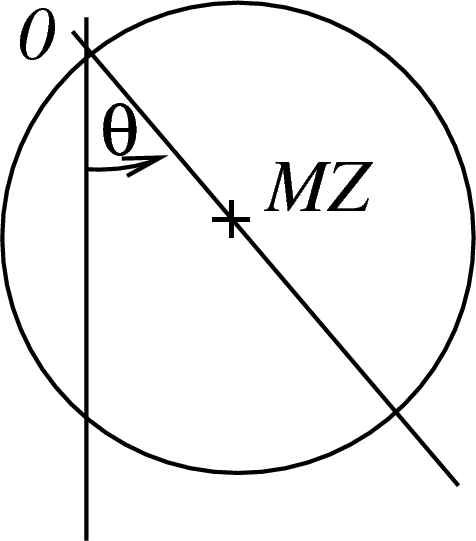
\includegraphics [width=0.8\linewidth]{irudiak/08a-orria-pendufisikoa.png}
\end {minipage}
}


\item
\raisebox{-0.8cm}{
\begin{minipage}{0.10\linewidth}
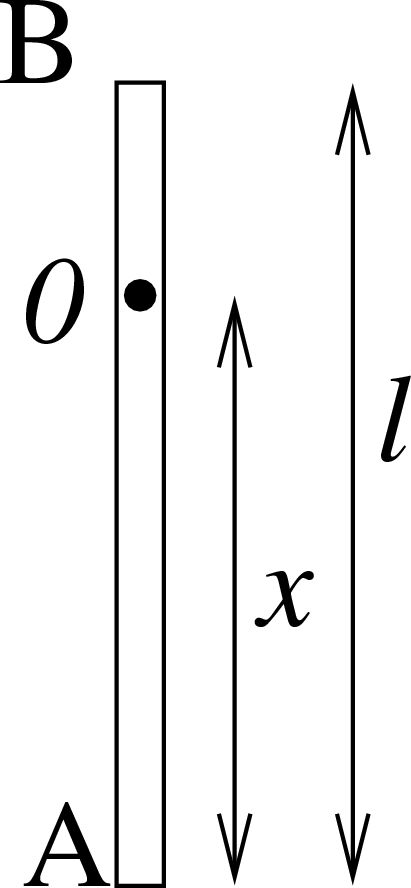
\includegraphics [width=\linewidth]{irudiak/08a-orria-makila.png}
\end {minipage}
\hspace*{0.5cm}
\begin{minipage}{0.80\linewidth}
 Makila astun bat $O$ puntutik zintzilikaturik dago eta bertikalaren
inguruan oszilatzen ari da, $O$-tik pasatzen den ardatz horizontal baten
inguruan oszilazio txikiak eginez. Zenbatekoa izan beharko du irudian
adierazitako $x$ distantziak, oszilazioen periodoa minimoa izan dadin?
\end {minipage}
}


\item
\raisebox{-1.3cm}{
\begin{minipage}{0.80\linewidth}
 Objektu lau batek $I$ inertzia-momentua du bere masa-zentruarekiko
(planoaren perpendikularra den ardatz batekiko). $P_1$ puntuaren inguruan
biratzean (ikus irudia), $T$ periodoaz oszilatzen ari da. Masa-zentruaren beste
aldean beste puntu bat aurki daiteke, $P_2$, berorrekiko oszilazioen periodoa
ere $T$ delarik. Froga bedi $P_1$ eta $P_2$ puntuen arteko distantzia
$gT^2/(4\pi^2)$ dela.
\end {minipage}
\hspace*{0.5cm}
\begin{minipage}{0.15\linewidth}
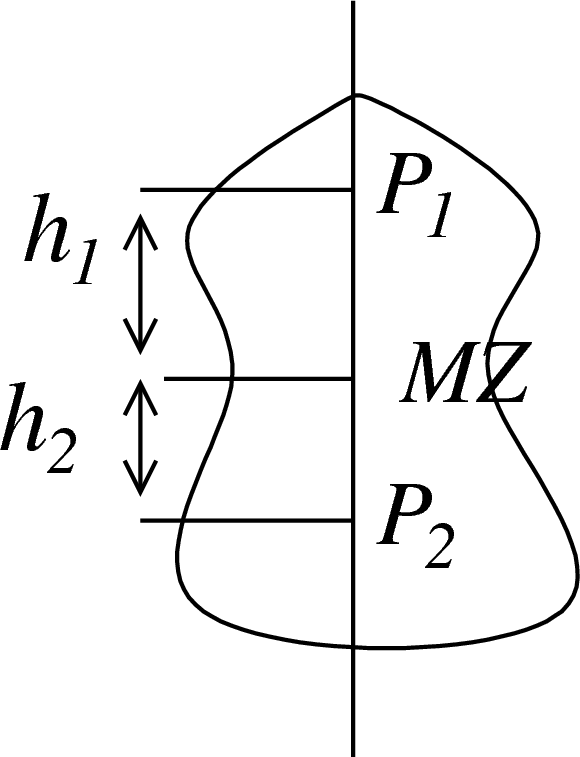
\includegraphics [width=\linewidth]{irudiak/08a-orria-P1P2.png}
\end {minipage}
}

\item
 Pendulu sinple baten periodoak $2.5\,{\rm s}$ balio du, oszilazio
txikiak egitean. Une batean oszilazioen anplitudeak $2^o$ balio izan du.
Marruskaduraren kausaz, anplitudea txikiagotuz joan da, 10 oszilazio
oso burutu ondoren $1.5^{\rm o}$-ko balioa hartzen duelarik. Lor bedi
indargetze-konstantearen balioa.


\item
Oszilatzaile harmoniko indargetuaren lasaikuntza-denbora honako hau
dugu: $\tau=1/(2\gamma)$, $\gamma$ delakoa indargetze-konstantea izanik.
Zeintzuk dira hala definituriko lasaikuntza-denboraren unitateak? Zenbatekoa da
$\tau$ denbora-tartea iragan ondoren oszilatzailearen anplitudeak jasaten duen
aldakuntza?


\end{enumerate}

{\bf Emaitzak }

%\begin{multicols}{2}{
\begin{enumerate}
\item[1.] $a$) x$\le0,031$~m; $b$) $\nu_{max}$=3,16~s$^{-1}$
\item[2.] $T=\frac{4}{\sin\alpha}\sqrt{\frac{2h_o}{g}}$
%\item[3.] $\bar{x}$=0; $\bar{x^2}=\frac{1}{2}A^2$
\item[4.] $K_{par}=k_1+k_2$; $\frac{1}{K_{ser}}=\frac{1}{k_1}+\frac{1}{k_2}$
\item[5.] a)$h_{max}=$17~mm, b)=0.26~s, d)0,54~m/s
\item[6.] $x$= 3,97~m
\item[7.] A=65~cm
\item[8.]  $\omega=\sqrt{g/(\rho_r a)}$
\item[9.] a)$A$=5~cm, $f$=1.58~Hz, $T=0,6347$~s b) $v_{max}$=0.495~m/s, t=0.158~s
   d) $\varphi$= 2.26~rad, $A$=3.91~cm
\item[11.] $T=2\pi\sqrt{\frac{2R}{g}}$; ($I=2MR^2$)
\item[12.] $x=l\frac{3+\sqrt{3}}{6}$; ($I=\frac{1}{12}ml^2+m(x-l/2)^2))$
\item[14.] $\gamma$=0,0115 s$^{-1}$
\item[15.] 0,606

\end{enumerate}
%}\end{multicols}


\end {document}
